\chapter{Fundamentos y Estado del Arte}
\label{ch:fundamentos}
Capítulo dedicado a describir los fundamentos y el panorama actual del trabajo. 

\section{Conceptos generales}
\label{se:ConceptosGeneralesa}

El concepto de NILM desde su introducción ha sido el método preferido por ingenieros e investigadores para la disgregación de consumo eléctrico desde su introducción, debido a sus ventajas económicas y prácticas.\autocite[pág. 2, pár. 4]{Nalmpantis2019}

En cuanto al origen de este método, se buscó categorizar en \autocite{192069} los dispositivos dentro de tres grandes grupos, para poder estructurar los diferentes dispositivos y generalizar el modelado de dispositivos específicos. 
Estos grupos son: 

\begin{enumerate}
\item \textbf{Señales de estados fijos} Siguen la arquitecturea de una máquina de estados finita, las transiciones entre estados son consumos exactos, al igual que los estados
\item \textbf{Señales transitorias} Esto son señales que no se encuentran en un espacio discreto que permita modelar su comportamiento como una máquina de estados. Un ejemplo podría ser un calefactor automático, que regula su generación de calor en función de la diferencia de la temperatura ambiente y la temperatura objetivo.
\item \textbf{Otras} Señales que no pueden categorizarse en ninguno de los dos casos anteriores. Por ejemplo, los cambios de dirección del motor de una lavadora en el proceso de lavado. 
\end{enumerate}

Cabe mencionar que los propios investigadores reconocieron que en el futuro los dispositivos eléctricos que siguiesen un diseño de máquinas de estados perderían precedencia. Ya que habría más 'dispositivos inteligentes' \autocite{192069}. Actualmente, una calefacción programable o un aire acondicionado programable están al alcance de cualquiera.
En 2021, en España el 50\% de las viviendas en alquiler constan de aire acondicionado\autocite{idealista2021}. 

Y esto es sólo un dispositivo. Habrá cientos de modelos de cada dispositivo, decenas de marcas, cada dispositivo con sus características específicas. 
Un modelado exhaustivo sería prácticamente imposible de crear y mantener, ya que sólo para el mercado doméstico hay una cantidad desorbitante de dispositivos, combinaciones de dispositivos, etc.

\subsubsection{Un ejemplo de sistema NILM}
Un sistema NILM consta de las siguientes partes: Una fuente de datos (acometida principal). Un dispositivo de recogida de datos (puede ser de Potencia Activa Y reactiva, Voltaje e Intensidad, etc). El modelo predictivo. Y el sistema de consulta de datos, que se ha omitido en la Figura \ref{diagramaNILM}.
\begin{figure}
    \centering
    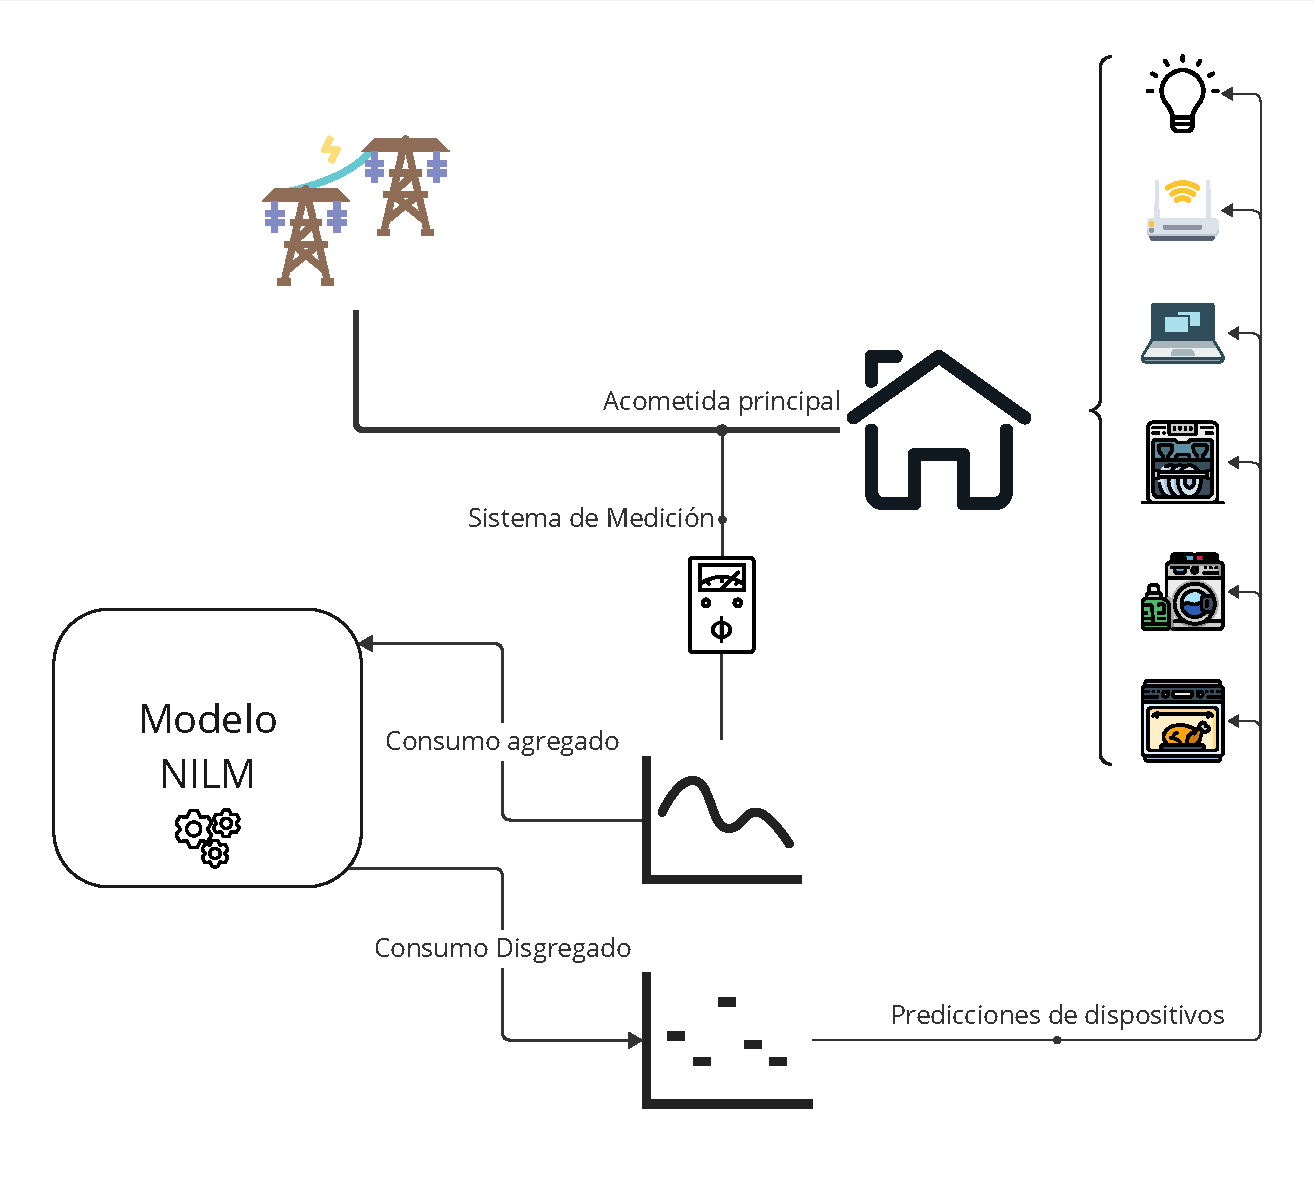
\includegraphics[width=450px]{images/SistemaNILM.pdf}
    \caption{Un diagrama simple de un sistema NILM}
    \label{diagramaNILM}
\end{figure}

Debido a estos argumentos, la investigación de la monitorización no intrusiva se inclinó a los modelos heurísiticos y el aprendizaje automático.
\todo[inline]{repasar motivos para el transfer learning}


\section{Aprendizaje Automático}

En la Historia de la Inteligencia Artificial, se han definido una serie de etapas de gran crecimiento y financiación como  \foreignquote{spanish}{veranos} (tres concretamente). Alternados por (dos) \foreignquote{spanish}{inviernos}; donde el interés, la financiación y el número de publicaciones decrecían significativamente \autocite{briefAIHistory}.
En los principios de la década de los 2010, comenzó el tercer \enquote{verano} de la Inteligencia Artificial. En 2012 ocurre un avance técnico: unos años antes, Olga Russakovsky creó el reto ImageNet \autocite{ImageNetRussakovsky}; un repositorio de más de un millón de imágenes de objetos a lo largo de más de mil categorías diferentes. 
Este reto estimuló a la comunidad científica, 

Resulta lógico que el número de artículos científicos proponiendo modelos que permitiesen resolver los retos que presenta NIML aumentase.


De los que voy a destacar los Modelos Ocultos de Markov, el Sparse Coding y finalmente las Redes Neuronales. Siendo estas últimas el foco principal del trabajo, y de este capítulo. 



\subsubsection{Identificando Datos Ocultos Con Cadenas de Markov}
Una cadena de Markov resulta útil cuando tenemos que modelar un comportamiento en base a una secuencia de eventos observables, siendo L.E. Baum y Ted Petrie los autores de \autocite{introductorHMM}, el primero de una serie de papers sobre modelos probabilísticos y estadística que introdujeron los HMM.
Estos eventos observables son elementos conocidos, pero la secuencia de estados del modelo para esos eventos observables son desconocidos. 

El problema, como en NILM, es que los estados no son directamente observables. Estan \textit{ocultos} y por tanto debemos ajustar la cadena para incluir una secuencia de posibles similitudes observadas \autocite{markovStandford}. 

En el caso de una cadena de Markov. Dados una serie de eventos observables, podemos inferir la probabilidad de cada estado que causaron estos eventos observables: Calculando la probabilidad de una cadena de eventos observables dada la probabilidad de una cadena de estados del conjunto, para todas las posibles combinaciones de la cadena los estados del conjunto. 
Este algoritmo se conoce algoritmo de Viterbi.

Este es el modelado que nos permite inferir de manera probabilística.
Cabe añadir que las cadenas de markov tienen una serie de algoritmos para determinar la cadena de estados ocultos más probable para la cadena de eventos observables, se omite por brevedad, pero puede consultarse \autocite{markovStandford} para una excelente y detallada explicación sobre este área.

\subsubsection{Modelos Ocultos de Markov}
Explicadas brevemente las bases de los Modelos Ocultos de Markov, pasamos a la aplicación de este modelo estadístico en la disgregación de consumos. 

Dado que un modelo de markov oculto infiere probabilísticamente una serie de estados, esto nos resulta útil para la disgregación de dispositivos. Para codificar diferentes estados de diferentes dispositivos se aumenta el número de cadenas del modelo. Teniendo una matriz de estados $S_i^j$ donde $S$ es un conjunto de estados; las observaciones dependen de todos los estados en un momento dado. Podemos observar esto en el siguiente diagrama:

Los Modelos de Markov Ocultos se han tratado en la literatura como efectivos en comparación con otras técnicas de monitorización cuando el entrenamiento supervisado presenta una baja tasa de muestreo en el eje temporal de la obtención de datos \autocite{frenchHMMNILM}.
Otras ventajas que presenta es su bajo coste computacional en el entrenamiento. Pero el uso de este tipo de elementos lo vuelven altamente susceptible a máximos locales\autocite{NILMreview2017}.

En el caso de los Modelos Factoriales de Markov Ocultos (con siglas FHMM en inglés), presentan ciertas ventajas en comparación con los HMM \footnote{Hidden Markov Models, o en español los Modelos Ocultos de Markov}:
La complejidad y el coste computacional de los los algoritmos de aprendizaje e inferencia son menores para los HMM. Sin embargo, tanto FHMM como HMM presentan limitaciones al volumen máximo de dispositivos simultáneos, incluso en casos como \autocite{afmap2012} donde se propone un nuevo algoritmo no supervisado. El algoritmo desarrollado (AFMAP) no presenta los problemas de alta complejidad y máximos locales, pero requiere de etiquetación manual después de la disgregación. Y presenta bajo rendimiento para dispositivos electrónicos y de cocina \autocite[5]{NILMreview2017}.

\section{Redes Neuronales}

En esta sección se tratan tres conceptos de las Redes Neuronales; se dará una introducción y se expondrán las aplicaciones pertinentes al tema del proyecto.
Por motivos de brevedad, se asume que el lector tiene una cierta base en inteligencia artificial. En caso contrario, sugiero consultar las citas y el \autoref{ch:anexoa}
\subsection{Sparse Coding}
Introducido por Olshausen et al.,1997 \autocite{OLSHAUSEN}. El Sparse Coding consiste en reducir la activación de la capa oculta de las neuronas, forzando a la red neuronal a realizar un aprendizaje \autocite{stanfordSparse}.
Su objetivo es encontrar un conjunto de vectores $\phi_i$ tal que podamos representar un vector $x$ como una combinación lineal de estos vectores: 
$$
x = \sum_{i=1}^{k}a_i\phi_i
$$
Este es un concepto que está fuertemente relacionado con los autoencoders y el aprendizaje PCA. 

Que tienen como objetivo es que su salida sea igual a la entrada, pero limitando la capa oculta para forzar un aprendizaje \autocite{stanfordAutoEncoding}.
Por ejemplo, supongamos que buscásemos utilizar un autoencoder para comprimir una imagen para enviarla por internet. Si no implementásemos restricciones, dado que el objetivo de la red neuronal es reducir la pérdida de información a 0; la salida del autoencoder sería la imagen, completamente idéntica.

Para evitar esto en el caso de los autoencoders se introduce una capa oculta de menor tamaño en comparación a la capa de entrada como restricción para forzar un aprendizaje, al tener una capa oculta, la capa de salida (de igual tamaño a la de entrada) debe \enquote{reconstruir} la entrada \autocite{stanfordAutoEncoding} .

Volviendo al Sparse Coding. Al tener un conjunto de vectores sobrecompleto, los coeficientes $a_i$ ya no se determinan únicamente por el vector de entrada $x$. Luego se define una función de escasez\footnote{De ahí el \enquote{Sparse}; escasez en Español}. Definimos esta función de escasez como: tener los menos componentes ($a_i$) distintos de cero o el mínimo de componentes no cerca de cero \autocite{stanfordSparse}.

Tanto los autoencoders como el sparse coding han sido usados en la literatura NILM.
sparse coding:\autocite{SparseCodingNILM}
\todo[inline]{Pendiente continuar investigando}

\subsection{Clasificadores de imágenes}
\todo[inline]{hablar de proyectos que usen clasificadores?}

\subsection{Redes Recurrentes}
\todo[inline]{hablar de proyectos que hagan uso de redes recurrentes}

\section{SOTA}
\subsection{Codificación GAF} 
La codificación elegida está motivada por \todo[inline]{cita pendiente} 
\subsection{CSPNet}     
\todo[inline]{entrar en detalle sobre CSPNet, sus creadores y proyectos SOTA que hagan uso de CSPNet}

\subsection{Validación de Modelos: NILMTK}  
\todo[inline]{hablar potencial implementación a futuro en nilmtk y papers que citan nilmtk}
